
\section{The Type System}
\label{infe}

In this section, we introduce the formal definition of our type system for numerical accuracy.
First, in Section \ref{secdeftypes}, we define the syntax of expressions and types and we introduce a set 
of inference rules.
Then we define in Section \ref{secdefprim} the types of the primitives for the operators among real numbers (addition, product, etc.)
These types are crucial in our system since they encode the propagation of the numerical
accuracy information.

\subsection{Expressions, Types and Inference Rules}
\label{secdeftypes}

In this section, we introduce the expressions, types and typing rules for our language.
For the sake of simplicity, the syntax introduced hereafter uses notations \textit{\`a la} lambda calculus
instead of the \texttt{ML}-like syntax employed in Section \ref{over}.
In our system, expressions and types are mutually dependent. They are defined inductively using the grammar of Equation (\ref{eqsyntax}).
\begin{equation}\label{eqsyntax}
\begin{array}{rcl}
\mathsf{Expr}\ni e&::=&\ \mathtt{r}\{s,u,p\}\in \mathsf{Real}_{u,p}\ |\ \mathtt{i}\in \mathsf{Int}
\ |\ \mathtt{b}\in \mathsf{Bool}\ |\ \mathtt{id}\in\mathsf{Id} \\
&&|\  \mathtt{if}\ e_0\ \mathtt{then}\ e_1\ \mathtt{else}\ e_2
\ |\ \lambda x.e
\ |\ e_0\ e_1\ |\ \mathtt{rec}\ f\ x.e\ |\ t\\
&&\\
\mathsf{Typ}\ni t&::=&|\ \mathtt{int}\ |\ \mathtt{bool}\ |\ \mathtt{real\{}i_0,i_1,i_2\mathtt{\}}\ |\ \alpha\ |\ \Pi x:e_0.e_1\\ 
&&\\
\mathsf{IExp}\ni i&::=&|\ \mathtt{int}\ |\ \mathtt{op}\in\mathsf{Id}_\mathsf{I}\ |\ \alpha
\ |\ i_0\ i_1
\end{array}
\end{equation}
In Equation (\ref{eqsyntax}), the $e$ terms correspond to expressions.
Constants are integers $\mathtt{i}\in \mathsf{Int}$, booleans $\mathtt{b}\in \mathsf{Bool}$ and real 
numbers  $\mathtt{r}\{s,u,p\}$ where $\mathsf{r}$
is the value itself, $s\in \mathsf{Sign}$ is the sign and $u,p\in \mathsf{Int}$ the $\mathsf{ufp}$ (see
Equation (\ref{equfp}))
and precision of $\mathtt{r}$. 
We have $\mathsf{Sign}=\{0,\oplus,\ominus,\top\}$ and $\mathsf{sign(r)}=0$ if $\mathsf{r}=0$,
$\mathsf{sign(r)}=\oplus$ if $\mathsf{r}>0$ and $\mathsf{sign(r)}=\ominus$ if $\mathsf{r}<0$.
The set $\mathsf{Sign}$ is equipped with the partial order relation $\prec\subseteq \mathsf{Sign}
\times \mathsf{Sign}$ defined by $0\prec \oplus$, $0\prec \ominus$, $\oplus\prec \top$ and 
$\ominus\prec \top$. The term $p$ defines the precision of $\mathsf{r}$. Let $\eps(\mathsf{r})$
be the absolute error on $\mathsf{r}$, we assume that
\begin{equation}
\eps(\mathsf{r})< 2^{u-p+1}\enspace .
\end{equation}
The errors on the numerical constants arising in programs are specified by the user or determined by default by 
the system. The errors on the computed values can be inferred by  propagation of the
initial errors.


\begin{figure}[tb]
\hrule
\vspace{0.1cm}
$$
\frac{}
     {\Gamma \vdash \texttt{i} :\ \mathtt{int} }\quad\textsc{(Int)}
	 \hspace{2cm}
\frac{}
     {\Gamma \vdash \texttt{b } :\ \mathtt{bool} }\quad\textsc{(Bool)}
$$

$$
\frac{\mathsf{sign}(\texttt{r}) \prec s\quad \mathsf{ufp}(\texttt{r})\le u}
     {\Gamma \vdash \texttt{r\{s,u,p\}}\ :\ \F{s}{u}{p} }\quad\textsc{(Real)}
\hspace{2cm}
\frac{\Gamma(\mathtt{id})=t}
     {\Gamma \vdash \mathtt{id}\ :\ t }\quad\textsc{(Id)}
$$

$$
\frac{
\Gamma \vdash e_0\ :\ \mathtt{bool}\hspace{1cm}\Gamma \vdash e_1\ :\ t_1\hspace{1cm} \Gamma \vdash e_2\ :\ t_2
\hspace{1cm} t=t_1\sqcup t_2}
{\Gamma\vdash \mathtt{if}\ e_0\ \mathtt{then}\ e_1\ \mathtt{else}\ e_2\ :\  t}\quad\textsc{(Cond)}
$$

$$
\frac{\Gamma,x :t_1 \vdash e :  t_2}
     {\Gamma \vdash \lambda x.e : \Pi x:t_1 .  t_2}\quad\textsc{(Abs)}
$$

$$
\frac{\Gamma \vdash e_1 : \Pi x: t_0. t_1\hspace{1cm} \Gamma \vdash e_2 :  t_2
\hspace{1cm} t_2\sqsubseteq t_0
}
     {\Gamma \vdash e_1\ e_2 :  t_2[x\mapsto e_2]}\quad\textsc{(App)}
$$

$$
\frac{\Gamma,x :t_1,f:\Pi.y:t_1.t_2  \vdash e :  t_2}
     {\Gamma \vdash \mathtt{rec}\ f\ x.e : \Pi x:t_1 .  t_2}\quad\textsc{(Rec)}
$$
\vspace{0.1cm}
\hrule
\caption{\label{figtyp}Typing rules for our language.} 
\end{figure}


In Equation (\ref{eqsyntax}), 
identifiers belong to the set $\mathsf{Id}$ and we assume a set of pre-defined identifiers 
$+$, $-$, $\times$, $\le$, $=$, $\ldots$ related to
 primitives for the logical and arithmetic operations.
We write $+$, $-$, $\times$ and $\div$ the operations on real numbers and
  $+\_$, $-\_$, $\times\_$ and $\div\_$ the operations among integers.
The language also admits conditionals, functions $\lambda x.e$, 
applications $e_0\ e_1$ and recursive functions $\texttt{rec}\ f\ x.e$ where
$f$ is the name of the function, $x$ the parameter and $e$ the body.
The language of expressions also includes type expressions $t$ defined by the second production of the grammar 
of Equation (\ref{eqsyntax}).

The definition of expressions and type is mutually recursive.
 Type variables are denoted $\alpha$, $\beta$, $\ldots$
and $\Pi x:e_0.e_1$ is used to introduce dependent types \cite{Pie04}. 
Let us remark that our language does not explicitly contain function types $t_0 \rightarrow t_1$
since they are encoded by means of dependent types. Let $\equiv$ denote the syntactic equivalence, we have
\begin{equation}
t_0\rightarrow t_1  \equiv \Pi x:t_0.t_1\quad\text{with}\ x\ \text{not free in}\ e\enspace .
\end{equation}
For convenience, we also write $\lambda x_0.x_1\ldots x_n.e$ instead of
$\lambda x_0.\lambda x_1\ldots\lambda x_n.e$ and 
$\Pi x_0:t_0.x_1:t_1\ldots x_n:t_n.e$ instead of
$\Pi x_0:t_0.\Pi x_1:t_1\ldots \Pi x_n:t_n.e$.

The types of constants are $\mathtt{int}$, $\mathtt{bool}$ and $\mathtt{real\{}i_0,i_1,i_2\mathtt{\}}$ 
where $i_0$, $i_1$ and $i_2$ 
are integer expressions
denoting the format of the real number. Integer expressions of $\mathsf{IExpr}\subseteq\mathsf{Expr}$ 
are a subset of expressions made of integer numbers, integer primitives of 
$\mathsf{Id}_\mathsf{I}\subseteq \mathsf{Id}$ (such as $+\_$, $\times\_$, etc.), type variables and applications.
Note that this definition restricts significantly the set of expressions which may be written inside
\texttt{real} types.

The typing rules for our system are given in Figure \ref{figtyp}. These rules are mostly classical.
The type judgment $\Gamma\vdash e : t$ means that in the type environment $\Gamma$, the expression
$e$ has type $t$. A type environment $\Gamma : \mathsf{Id}\rightarrow\mathsf{Typ}$ map identifiers to types.
We write $\Gamma\ x:t$ the environment $\Gamma$ in which the variable $x$ has type $t$.
The typing rules \textsc{(Int)} and \textsc{(Bool)} are trivial. Rule \textsc{(Real)} states that
the type of a real number $\texttt{r\{s,u,p\}}$ is  $\F{s}{u}{p}$ assuming that the
actual sign of \texttt{r} is less than $s$ and that the \textsf{ufp} of \texttt{r} is less than $u$.
Following Rule \textsc{(Id)}, an identifier \texttt{id} has type $t$ if $\Gamma(\mathtt{id})=t$.
Rules \textsc{(Cond)}, \textsc{(Abs)} and \textsc{(Rec)} are standard rules for conditionals and abstractions respectively.
The rule for application, \textsc{(App)}, requires that the first expression $e_1$ has type
$\Pi x: t_0. t_1$ (which is equivalent to $t_0\rightarrow t_1$ if $x$ is not free in $t_1$)
and that the argument $e_2$ has some type $t_2\sqsubseteq t_0$. The sub-typing relation $\sqsubset$
is introduced for real numbers. Intuitively, we want to allow the argument of some function
to have a smaller \textsf{ulp} than what we would require if we used $t_0=t_2$ in Rule
\textsc{(App)}, provided that the precision $p$ remains as good with $t_2$ as with $t_0$.
This relaxation allows to type more terms without invalidating the type judgments.
Formally, the relation $\sqsubseteq$ is defined in Equation (\ref{eqlttype}).
\begin{equation}\label{eqlttype}
\F{s_1}{u_1}{p_1} \sqsubseteq \F{s_2}{u_2}{p_2} \iff s_1\sqsubseteq s_2\ \wedge\ u_2 \ge u_1\ \wedge\ p_2 \ge u_1 - u_2 + p_1
\end{equation}
In other words, the sub-typing relation of Equation (\ref{eqlttype}) states that it is
always correct to add zeros before the first significant digit of a number, as illustrated in
Figure \ref{figlt}.
 

\begin{figure}[tb]
  \begin{center}
\hrule
\vspace{0.1cm}
    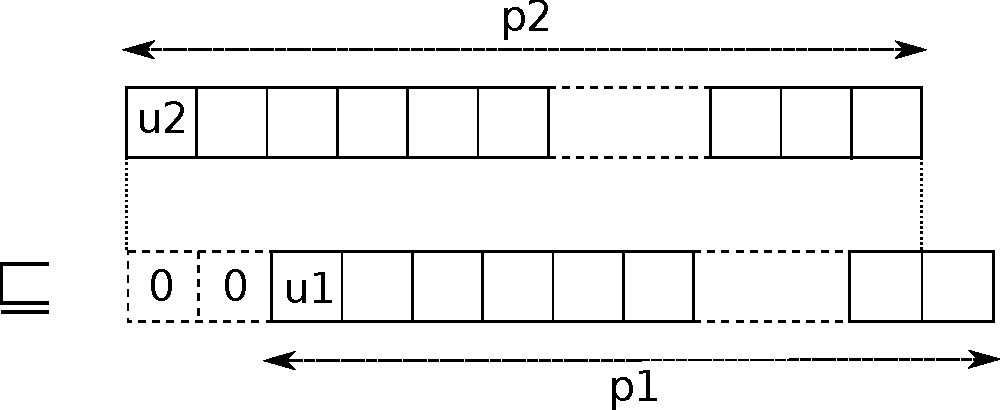
\includegraphics[width=6.5cm]{lttype.pdf}
\vspace{0.1cm}
\hrule
    \caption{    \label{figlt}The sub-typing relation $\sqsubseteq$ of  Equation (\ref{eqlttype}).}
  \end{center}
\end{figure}

\subsection{Types of Primitives}
\label{secdefprim}

In this section, we introduces the types of the primitives of our language.
As mentionned earlier, the arithmetic and logic operators are viewed as functional constants of the language. 
The type of a primitive for an arithmetic operation among integers $\ast\_  \in\{+\_, -\_,\times\_,\div\_\}$ is
\begin{equation}\label{eqtypint}
t_{\ast\_}=\Pi x:\texttt{int}.y:\texttt{int}.\texttt{int}\enspace .
\end{equation}
The type of comparison operators $\Join\in\{=,\not=,<,>,\le,\ge\}$ are polymorphic with the restriction
that they reject the type $\F{s}{u}{p}$ which necessitates special comparison operators:
\begin{equation}\label{eqtyprel}
t_{\Join}=\Pi x:\alpha.y:\alpha.\texttt{bool}\quad \alpha\not=\F{s}{u}{p}\enspace .
\end{equation}
For real numbers, we use comparisons at a given accuracy defined by the operators $\Join_{\{u,p\}}\in
\{<_{\{u,p\}},>_{\{u,p\}}\}$. We have
$$
\begin{array}{c}
t_{\Join_{\{u,p\}}} = \Pi \mathtt{s}:\texttt{int},\mathtt{u}:\texttt{int}, \mathtt{p}:\texttt{int},
\mathtt{s}:\texttt{int}, \mathtt{u}:\texttt{int}, \mathtt{p}:\texttt{int}.\\
\hspace{0.8cm}\F{s}{u}{p+1}\rightarrow\F{s}{u}{p+1}
\rightarrow\mathtt{bool}
\end{array}\enspace .
$$
Remark that the operands of a comparison $\Join_{\{u,p\}}$ must have $p+1$ bits of accuracy.
This is to avoid unstable tests, as detailed in the proof of Lemma \ref{wsubject} in Section \ref{correct}. 
An unstable test is a comparison between two approximate values
such that the result of the comparison is falsened by the approximation error.
For instance, if we reuse an example of Section \ref{over}, in IEEE754 double precision,
the condition $10^{16}+1=10^{16}$ evaluates to \texttt{true}. We need to avoid such situations
in our language in order to preserve our subject reduction theorem (we need the control-flow
be the same in the finite precision and exact semantics).
Let us also note
that our language does not prodive an equality relation $=_{\{u,p\}}$ for \texttt{real} values.
Again this is to avoid unstable tests. Given values $x$ and $y$ of type $\F{s}{u}{p}$,
the programmer is invited to use $|x-y|<2^{u-p+1}$
instead of $x=y$ in order to get rid of the perturbations introduced by the finite precision arithmetic.

%$$
%\begin{array}{c}
%\texttt{+} : \Pi u_1:\texttt{int}. \Pi p_1:\texttt{int}.\Pi u_2:\texttt{int}. \Pi p_2:\texttt{int}.\\
%\quad\F{s_1}{u_1}{p_1}\rightarrow\F{s_2}{u_2}{p_2}\rightarrow\F{??}{u_1+u_2+1}{u_1+u_2+1-\max\big(\mathtt{u_1}-\mathtt{p_1},\mathtt{u_2}-\mathtt{p_2}\big)
%-\iota\big(\mathtt{u_1}-\mathtt{p_1},\mathtt{u_2}-\mathtt{p_2}\big)
%}
%\end{array}
%$$


\begin{figure}[tb]
\hrule			
$$
\begin{array}{c}
\ast\in\{ +,-,\times,\div\}\\
\\
\mathtt{t_\ast} = \Pi \mathtt{s_1}:\texttt{int},\mathtt{u_1}:\texttt{int}, \mathtt{p_1}:\texttt{int},\mathtt{s_2}:\texttt{int}, \mathtt{u_2}:\texttt{int}, \mathtt{p_2}:\texttt{int}.\\
\hspace{0.8cm}\F{s_1}{u_1}{p_1}\rightarrow\F{s_2}{u_2}{p_2}\\
\hspace{3.2cm}
\rightarrow\F{\mathcal{S}_\ast(\mathtt{s_1},\mathtt{u_1},\mathtt{s_2},\mathtt{u_2})}
{\mathcal{U}_\ast(\mathtt{s_1},\mathtt{u_1},\mathtt{s_2},\mathtt{u_2})}
{\mathcal{P}_\ast(\mathtt{s_1},\mathtt{u_1},\mathtt{p_1},\mathtt{s_2},\mathtt{u_2},\mathtt{p_2})}
\end{array}
$$
%\small
$$
\begin{array}{rcl}
\mathcal{U}_+(\mathtt{s_1},\mathtt{u_1},\mathtt{s_2},\mathtt{u_2}))&=&\max(\mathtt{u_1},\mathtt{u_2})
+\sigma_+(\mathtt{s_1},\mathtt{s_2})\\
\mathcal{P}_+(\mathtt{s_1},\mathtt{u_1},\mathtt{p_1},\mathtt{s_2},\mathtt{u_2},\mathtt{p_2}) &=&
\max(\mathtt{u_1},\mathtt{u_2})+\sigma_+(\mathtt{s_1},\mathtt{s_2})-
   \max(\mathtt{u_1}-\mathtt{p_1},\mathtt{u_2}-\mathtt{p_2})-\iota(\mathtt{u_1}-\mathtt{p_1},\mathtt{u_2}-\mathtt{p_2})\\
   \\
\mathcal{U}_-(\mathtt{s_1},\mathtt{u_1},\mathtt{s_2},\mathtt{u_2})) &=&\max(\mathtt{u_1},\mathtt{u_2})
+\sigma_-(\mathtt{s_1},\mathtt{s_2})\\
\mathcal{P}_-(\mathtt{s_1},\mathtt{u_1},\mathtt{p_1},\mathtt{s_2},\mathtt{u_2},\mathtt{p_2}) &=&
\max(\mathtt{u_1},\mathtt{u_2})+\sigma_-(\mathtt{s_1},\mathtt{s_2})-
   \max(\mathtt{u_1}-\mathtt{p_1},\mathtt{u_2}-\mathtt{p_2})-\iota(\mathtt{u_1}-\mathtt{p_1},\mathtt{u_2}-\mathtt{p_2})\\
\\
\\
\mathcal{U}_\times(\mathtt{s_1},\mathtt{u_1},\mathtt{s_2},\mathtt{u_2}))&=&\mathtt{u_1}+\mathtt{u_2}+1\\
\mathcal{P}_\times(\mathtt{s_1},\mathtt{u_1},\mathtt{p_1},\mathtt{s_2},\mathtt{u_2},\mathtt{p_2})&=&
\mathtt{u_1}+\mathtt{u_2}+1-
\max(
\mathtt{u_1}+\mathtt{u_2}+1-\mathtt{p_1},
\mathtt{u_1}+\mathtt{u_2}+1-\mathtt{p_2})-\iota(\mathtt{p_1},\mathtt{p_2})\\
\\
\mathcal{U}_\div(\mathtt{s_1},\mathtt{u_1},\mathtt{s_2},\mathtt{u_2}))&=&\mathtt{u_1}-\mathtt{u_2}+1\\
\mathcal{P}_\div(\mathtt{s_1},\mathtt{u_1},\mathtt{p_1},\mathtt{s_2},\mathtt{u_2},\mathtt{p_2})&=&\mathcal{P}_\times(\mathtt{u_1},\mathtt{p_1},\mathtt{u_2},\mathtt{p_2})-1\\
\\
\iota(x,y)&=&\left\{\begin{array}{l}
1 \ \text{if}\ x=y,\\
0\ \text{otherwise}.
\end{array}\right.
\end{array}
$$
\scriptsize
\vspace{0.2cm}
$$
\begin{array}{ccc}
\mathcal{S}_+&&\mathcal{S}_\times \ \text{and}\ \mathcal{S}_\div
\\
%%%%%%%%%%%%%%%%%%%%%%%%%%%%%%%%%%%%%%%%%%%%%
\begin{array}{c|c|c|c|c}
 \mathtt{s_1} \backslash \mathtt{s_2}
      &\quad 0 \quad& + & - & \quad\top\quad \\
  \hline	  
  \begin{array}{c}
  \\ 0\\ \\
  \end{array}    & 0 & + & - & \top \\
  \hline
  +    & + & + & 
  \begin{array}{c}
  + \ \text{if}\ \mathtt{u_1}<\mathtt{u_2}\\
  - \ \text{if}\ \mathtt{u_2}<\mathtt{u_1}\\
  \top\ \text{otherwise}
  \end{array}&\top\\
  \hline
  -     & - & 
  \begin{array}{c}
  + \ \text{if}\ \mathtt{u_2}<\mathtt{u_1}\\
  - \ \text{if}\ \mathtt{u_1}<\mathtt{u_2}\\
  \top\ \text{otherwise}
  \end{array}
  & - &\top\\
  \hline
  \begin{array}{c}
  \\ \top\\ \\
  \end{array} &\top &\top&\top&\top
\end{array}
&\hspace{1cm}&
\begin{array}{c|c|c|c|c}
   \mathtt{s_1} \backslash \mathtt{s_2}
      &\quad 0 \quad& \quad+\quad & \quad-\quad & \quad\top\quad \\
  \hline	  
  \begin{array}{c}
  \\ 0\\ \\
  \end{array}    & 0 & 0 & 0 & 0 \\
  \hline
  \begin{array}{c}
  \\ +\\ \\
  \end{array}    & 0 &  + & - &\top\\
  \hline
  \begin{array}{c}
  \\ -\\ \\
  \end{array}    & 0 & - & +  &\top\\
  \hline
  \begin{array}{c}
  \\ \top\\ \\
  \end{array} &0 &\top&\top&\top
\end{array}
\end{array}
 $$
\vspace{0.2cm}
 $$
 \begin{array}{ccc}
\mathcal{S}_-&&
\\
\begin{array}{c|c|c|c|c}
 \mathtt{s_1} \backslash \mathtt{s_2}
      &\quad 0 \quad& + & - & \quad\top\quad \\
  \hline	  
  \begin{array}{c}
  \\ 0\\ \\
  \end{array}    & 0 & - & + & \top \\
  \hline
  +    & + &  
  \begin{array}{c}
  - \ \text{if}\ \mathtt{u_1}<\mathtt{u_2}\\
  + \ \text{if}\ \mathtt{u_2}<\mathtt{u_1}\\
  \top\ \text{otherwise}
  \end{array}& +&\top\\
  \hline
  -     & - & - &
  \begin{array}{c}
  - \ \text{if}\ \mathtt{u_2}<\mathtt{u_1}\\
  + \ \text{if}\ \mathtt{u_1}<\mathtt{u_2}\\
  \top\ \text{otherwise}
  \end{array}
  &\top\\
  \hline
  \begin{array}{c}
  \\ \top\\ \\
  \end{array} &\top &\top&\top&\top
\end{array}
&\hspace{2.5cm}&
\begin{array}{cc}
\sigma_+&
\begin{array}{c|cccc}
  & 0 & + & - & \top \\
  \hline
0& 0 & 0  & 0 & 0 \\
+& 0 & 1 & 0 & 1\\
-& 0 & 0 & 1 & 1\\
\top&0&1 & 1 &1 
\end{array}
\\
&\\
\sigma_- &
\begin{array}{c|cccc}
  & 0 & + & - & \top \\
  \hline
0& 0 & 0  & 0 & 0 \\
+& 0 & 0 & 1 & 1\\
-& 0 & 1 & 0 & 1\\
\top&0&1 & 1 &1 
\end{array}
\end{array}
\end{array}
$$
\hrule
\caption{\label{figtypprim}Types of the primitives corresponding to the elementary arithmetic operations.} 
\end{figure}

 
The types of primitives for real arithmetic operators are fundamental in our system since they encode
the propagation of the numerical accuracy information. They are defined in Figure \ref{figtypprim}.
The type $t_\ast$ of some operation $\ast\in\{+,-,\times,\div\}$ is a pi-type with takes
six arguments $\mathsf{s_1,u_1,p_1,s_2,u_2}$ and $\mathsf{p_2}$ of type \texttt{int} corresponding to the sign, \textsf{ufp} and precision of
the two operands of $ast$ and which produces a type
\begin{equation}\label{eqrealtype}
\F{s_1}{u_1}{p_1}\rightarrow\F{s_2}{u_2}{p_2}
\rightarrow\F{\mathcal{S}_\ast(\mathtt{s_1},\mathtt{s_2})}
{\mathcal{U}_\ast(\mathtt{s_1},\mathtt{u_1},\mathtt{s_2},\mathtt{u_2})}
{\mathcal{P}_\ast(\mathtt{u_1},\mathtt{p_1},\mathtt{u_2},\mathtt{p_2})}\enspace .
\end{equation}
In Equation (\ref{eqrealtype}), $\mathcal{S}_\ast$, $\mathcal{U}_\ast$ and $\mathcal{P}_\ast$
are functions which compute the sign, \textsf{ufp} and precision of the result of
the operation $\ast$ in function of  $\mathsf{s_1,u_1,p_1,s_2,u_2}$ and $\mathsf{p_2}$.
These functions are also given in Figure \ref{figtypprim}. They extend the functions
used in \cite{Mar17}.

The functions $\mathcal{S}_\ast$
determine the sign of the result of an operation in function of the signs of the operands and,
for additions and subtractions, in function of the \textsf{ufp}'s of the operands.
The functions $\mathcal{U}_\ast$ compute the \textsf{ufp} of the result.
Remark that $\mathcal{U}_+$ and $\mathcal{U}_-$ use the functions $\sigma_+$ and $\sigma_-$,
respectively. These functions are defined in the bottom right corner of Figure \ref{figtypprim}
to increment the \textsf{ufp} of the result of some addition or subtraction in the relevant cases only.
For example if $a$ and $b$ are two positive real numbers then $\mathsf{ufp}(a+b)$ is possibly 
$\max\big(\mathsf{ufp}(a)+\mathsf{ufp}(b)\big)+1$ but if $a>0$ and $b<0$ then
$\mathsf{ufp}(a+b)$ is not greater than $\max\big(\mathsf{ufp}(a)+\mathsf{ufp}(b)\big)$.
The functions $\mathcal{P}_\ast$ compute the precision of the result. Basically,
they compute the number of bits between the \textsf{ufp} and the \textsf{ulp} 
of the result. 

We end this section by exhibiting some properties of the functions
$\mathcal{P}_\ast$. 
Let
$\eps(x)$ denote the error on $x\in\mathsf{Real}_{u,p}$. We have $\eps(x)< 2^{u-p+1}=\mathsf{ulp}(x)$.
Let us start with the addition. Lemma \ref{lemadd} relates the accuracy of the operands to the accuracy
of the result of an addition between two values $x$ and $y$.

\begin{lemma}\label{lemadd}
Let $x$ and $y$ be two values such that $\eps(x)< 2^{u_1-p_1+1}$ and $\eps(y)< 2^{u_2-p_2+1}$.
Let $z=x+y$ and let
\begin{equation}
\begin{array}{rcl}
u&=&\mathcal{U}_+(s_1,u_1,s_2,u_2)\enspace ,\\
p&=&\mathcal{P}_+(s_1,u_1,p_1,s_2,u_2,p_2)\enspace .
\end{array}
\end{equation}
Then 
\begin{equation}
\eps(z)<2^{u+p-1}\enspace .
\end{equation}
\end{lemma}

\begin{proof}

 The errors on the addition may be bounded
by $e_+=\eps(x)+\eps(y)$. 
Then the most significant bit of the error has weight $\mathsf{ufp}(e_+)$
and the accuracy of the result is $p=\mathsf{ufp}(x + y)-\mathsf{ufp}(e_+)$.
Let 
$$
u=\mathsf{ufp}(x+y)=\max(u_1,u_2)+\sigma_+(s_1,s_2)=\mathcal{U}_+(s_1,u_1,s_2,u_2)
$$
We need to over-approximate $e_+$ in order to ensure $p$. 
We have
$
\eps(x)< 2^{u_1-p_1+1}$ and $\eps(y)< 2^{u_2-p_2+1}
$
and, consequently,
$
e_+ < 2^{u_1-p_1+1}+  2^{u_2-p_2+1}.
$
We introduce the function $\iota(x,y)$ also
defined in Figure \ref{figtypprim} and which is equal to $1$ if $x=y$ and $0$ otherwise.
 We have
$$
\begin{array}{rcl}
\mathsf{ufp}(e_+) &<& \max(u_1-p_1+1,u_2-p_2+1)+\iota(u_1-p_1,u_2-p_2) \\
          &\le& \max(u_1-p_1,u_2-p_2)+\iota(u_1-p_1,u_2-p_2)
\end{array}$$
Let us write
\begin{equation}
p = \max(u_1-p_1,u_2-p_2)-\iota(u_1-p_1,u_2-p_2)=\mathcal{P}_+(s_1,u_1,p_1s_2,u_2,p_2)\enspace .
\end{equation}
We conclude that
$u=\mathcal{U}_+(s_1,u_1,s_2,u_2)$, $p=\mathcal{P}_+(s_1,u_1,p_1s_2,u_2,p_2)$ and
$\eps(z) < 2^{u+p-1}$
\end{proof}

Lemma \ref{lemprod} is similar to Lemma \ref{lemadd}  for the product. 

\begin{lemma}\label{lemprod}
Let $x$ and $y$ be two values such that $\eps(x)< 2^{u_1-p_1+1}$ and $\eps(y)< 2^{u_2-p_2+1}$.
Let $z=x\times y$ and let
\begin{equation}
\begin{array}{rcl}
u&=&\mathcal{U}_\times (s_1,u_1,s_2,u_2)\enspace ,\\
p&=&\mathcal{P}_\times (s_1,u_1,p_1,s_2,u_2,p_2)\enspace .
\end{array}
\end{equation}
Then 
\begin{equation}
\eps(z)<2^{u+p-1}\enspace .
\end{equation}
\end{lemma}


\begin{proof}
For the product, we have
$p	= \mathsf{ufp}(x\times y)-\mathsf{ufp}(e_\times)$ with $e_\times=x\cdot \eps(y)+y\cdot \eps(x)+\eps(x)\cdot\eps(y)$. 
Let
$$
u=u_1+u_2+1=\mathcal{U}_\times (s_1,u_1,s_2,u_2)\enspace .
$$

We have, by definition of $\mathsf{ufp}$,
$
2^{u_1} \le x < 2^{u_1+1}\quad\text{and}\quad 2^{u_2} \le y< 2^{u_2+1}\enspace.
$
Then $e_\times$ may be bound by
\begin{equation}\label{eqproof1}
\begin{array}{rcl}
e_\times &<& 2^{u_1+1}\cdot 2^{u_2-p_2+1} + 2^{p_2+1}\cdot 2^{u_1-p_1+1}+ 2^{u_1-p_1+1}\cdot 2^{u_2-p_2+1}\\
            &=& 2^{u_1+u_2-p_2+2}+ 2^{u_1+u_2-p_1+2}+ 2^{u_1+u_2-p_1-p_2+2} \enspace.
\end{array}
\end{equation}
Since $u_1+u_2-p_1-p_2+2< u_1+u_2-p_1+2$ and $u_1+u_2-p_1-p_2+2< u_1+u_2-p_2+2$, 
we may get rid of the last term of Equation (\ref{eqproof1}) and we
obtain that
$$
\begin{array}{rcl}
\mathsf{ufp}(e_\times) &<& \max(u_1+u_2-p_1+2,u_1+u_2-p_2+2)+\iota(p_1,p_2)\\
&\le & \max(u_1+u_2-p_1+1,u_1+u_2-p_2+1)+\iota(p_1,p_2)\enspace.
\end{array}
$$
Let us write
\begin{equation}
p = \max(u_1+u_2-p_1+1,u_1+u_2-p_2+1)-\iota(p_1,p_2)=\mathcal{P}_\times(s_1,u_1,p_1s_2,u_2,p_2)\enspace .
\end{equation}
We conclude that
$u=\mathcal{U}_\times(s_1,u_1,s_2,u_2)$, $p=\mathcal{P}_\times(s_1,u_1,p_1s_2,u_2,p_2)$ and
$\eps(z) < 2^{u+p-1}$
\end{proof}

Note that, by reasoning on the exponents of the values, the constraints resulting from a product become linear.
The equations for the subtraction and division are almost identical to the equations for the addition and product, 
respectively. Note that the result of a division has one less bit than the result of a product.
This is due to the fact that, even in the operands are finite numbers, the result of the
division may be irrational and possibly needs to be truncated.
We conclude this section with the following theorem which summarize the properties of the types
of the result of the four elementary operations.

\begin{theorem}\label{thop}
Let $x$ and $y$ be two values such that $\eps(x)< 2^{u_1-p_1+1}$ and $\eps(y)< 2^{u_2-p_2+1}$ and
let $\ast\in\{ +,-,\times,\div\}$ be an elementary operation.
Let $z=x\ast y$ and let
\begin{equation}
\begin{array}{rcl}
u&=&\mathcal{U}_\ast (s_1,u_1,s_2,u_2)\enspace ,\\
p&=&\mathcal{P}_\ast (s_1,u_1,p_1,s_2,u_2,p_2)\enspace .
\end{array}
\end{equation}
Then 
\begin{equation}
\eps(z)<2^{u+p-1}\enspace .
\end{equation}
\end{theorem}

\begin{proof}
The cases of the addition and product correspond to Lemma \ref{lemadd} and Lemma \ref{lemprod}, respectively.
The cases of the subtraction and  division are similar to the former ones.
\end{proof}



